\section{Example: Circuit Simulator}
\label{sec:ex}

In this section we give an overview of Legion using an example.
Listing~\ref{lst:code_ex} shows code for an electrical
circuit simulation, which illustrates the core features of the programming model.

The circuit simulation takes a collection of
of wires and nodes where wires meet.  
The simulation repeatedly updates
currents, distributes charges, and updates voltages for as many
time steps as the simulation demands.  We first
describe the partitioning of regions in Section~\ref{subsec:partitioning}
and then describe the data type declarations in Section~\ref{subsec:datatypes}.

\subsection{Regions and Partitions}
\label{subsec:partitioning}

Line 9 declares the main simulator function, which takes a {\tt
Circuit} to be simulated.  This function specifies the regions it 
accesses and the {\em privileges} and {\em coherence} it requires of those regions.
In this case, the {\tt RWE} annotation specifies that the function
accesses the regions {\tt c.r\_all\_nodes} and {\tt c.r\_all\_wires}
with read-write privileges and {\em exclusive} coherence (i.e., no other
function can access these two regions concurrently).  The simulation 
reads and writes all nodes and wires, and it must be done
with exclusive access to ensure correct results.  Privileges specify what
the function can do with the regions; coherence specifies what other
functions can do with the regions concurrently.  Functions that
declare their accessed regions, privileges, and coherence are called {\em tasks}
and are the unit of parallel execution in Legion.

Lines 15-21 are responsible for partitioning the circuit into {\tt MAX\_PIECES}
pieces that can be worked on in parallel.  To partition a region, we
provide a {\em coloring}, which is a relation between the elements
of a region and a set of colors.  A {\em partition} is an object which given
a coloring and a region $r$ contains for each color $c$ a {\em subregion} of $r$
containing all the elements of $r$ colored $c$.

Wires are simply partitioned in {\tt MAX\_PIECES} subregions (line 16).  
The nodes are first partitioned into 
{\em private} and {\em shared} nodes (line 21).  Private nodes
are touched by a single task in a phase, while shared nodes may
be referenced by multiple tasks in a phase.  The thick lines in Figure~\ref{sfig:part_fig:pvs}
show how the nodes in a small graph might be partitioned into three subsets.  Gray
nodes are shared and black nodes are private.  Note that
this partition is disjoint since each node has one color.
%Our current implementation uses small
%integers or booleans for the names of colors, but any enumerable set would be
%fine.  The coloring relation need not be total - it can leave out some elements entirely.  And although it is not required to be injective (it can map a single
%element to multiple colors), the fact that injective mappings will always
%result in disjoint subregions makes them strongly encouraged (when possible).
%Our example uses four colorings to create circuit partitions.

We next further partition the private and shared subregions into {\tt
  MAX\_PIECES} disjoint subregions each (lines 20-23); one subregion
of the private and shared node partitions is shown in
Figures~\ref{sfig:part_fig:p_i} and \ref{sfig:part_fig:s_i}
respectively.  

We partition the shared nodes a second time using a
different coloring into the sets of ghost nodes for each task.  This 
partition is noteworthy because the subregions are {\em not} disjoint:
ghost nodes may be read by multiple tasks, and thus a node $n$  may belong 
to more than one ghost region, which corresponds to $n$ being assigned
more than one color by the coloring {\tt node\_neighbor\_map}.
One of the ghost subregions is shown in Figure~\ref{sfig:part_fig:g_i}.

Figure~\ref{sfig:part_fig:tree} shows the final hierarchy of node
partitions;  the $*$ symbol indicates a partition is disjoint. This
{\em region tree} data structure plays an important role in scheduling
tasks for out-of-order execution (see Section~\ref{sec:soop}).


%(These subsets are hopefully reasonably compact, but the correctness
%of the simulation is not dependent on that.)  
%Once the subsets are known, the \emph{node\_owner\_map} is created by assigning
%each node the color corresponding to its subset.  The 
%\emph{wire\_owner\_map} assigns each wire to the same subset as its ``in\_node''.
%The \emph{node\_nghbr\_map} maps a node to color(s) of all wires that 
%connect to it.  Finally, the \emph{node\_sharing\_map} is derived from the
%\emph{node\_nghbr\_map}, with a node colored ``true'' if any colors other than 
%its own were used, and ``false'' if the only wires that connect to a node are
%in the same piece.
%Figure~\ref{fig:part_fig} shows how the partitions are defined.

%Line 19 uses the \emph{wire\_owner\_map} to partition the wires region of the
%circuit into a subregion for each piece, but the partitioning of the nodes is
%more complicated due to the sharing that is necessary between the pieces.
%First, the \emph{node\_sharing\_map} is used to create two subregions: $p\_nodes\_pvs[false]$ contains all the nodes that are private to some piece (i.e. will
%never be needed for the computations in any other piece), while $p\_nodes\_pvs[true]$ contains nodes that will be accessed by multiple pieces' computations.
%Each of these subregions is then partitioned using the $node\_owner\_map$ to
%create the subregions owned by each computation.  These are the $p_i$ and $s_i$
%subregions, shown in Figures \ref{sfig:part_fig:p_i} and \ref{sfig:part_fig:s_i}.  Finally, the $g_i$ subregions (shown in Figure~\ref{sfig:part_fig:g_i}) are
%created using the $node\_nghbr\_map$ to 
%create subregions that include the ``ghost'' nodes needed to perform each
%piece's calculations.

%With the partitioning operations completed, the various subregions are
%recorded in an array of {\tt CircuitPiece} structures.  Lines 32-33 fill in multiple
%fields of a {\tt CircuitPiece} at once.  The need for such a statement will be described in detail in 
%section \ref{subsec:datatypes}.

%Because a region relationship can have
%fields with types that refer its own fields' values, it is often not possible
%to assign fields one at a time without violating the type checking rules.
%The simultaneous assignment operator asks the type checker only to make sure
%that the fields in the structure would have the right (self-referential) types
%after all the fields have been changed.

Lines 31-57 form the bulk of the actual simulation, performing three passes
over the circuit in each iteration.  Each pass loops over an array of pieces (constructed on lines 27-30 from the partitions),
spawning a task for each piece.   There are no explicit requests for
parallel execution (the default semantics of {\tt spawn} is sequential 
execution of the spawned tasks) nor is there synchronization required between the
passes.  Both the fact that the tasks can be run in parallel within a pass
and the required inter-pass dependencies are determined automatically
by the Legion runtime based on the region access annotations on the task declarations
(see Section~\ref{sec:soop}).

%The declarations for the three subtasks are shown on lines 42-51.  
The  {\tt calc\_new\_currents} task reads and writes the wires subregion, 
the nodes subregion, and the ghost node region for its piece.
The {\tt distribute\_charge} subtask is a different phase that reads the piece's 
wires subregion and updates all nodes those wires touch.  However,
rather than requesting the ability to read and write the nodes (which would
require serialization of these tasks for correctness), the task declares that
it will use reorderable {\em reduction} operations and that the coherence requirement
is {\em atomic} rather than exclusive access. The final task is 
{\tt update\_voltages}, which writes the shared and private nodes for a piece
and reads the results of the previous task's reductions.

  
%Since the wire subregions are known to be disjoint,
%the write sets of invocations of $calc\_new\_currents$ do not overlap, and can
%therefore be safely run in parallel.


%As long as the
%runtime can guarantee to apply the reductions from multiple subtasks safely, it
%can run the subtasks themselves in parallel.  Each invocation of 
%$distribute\_charge$ will be delayed until the corresponding invocation of 
%$calc\_new\_currents$ has completed due to the read-after-write dependency on
%the corresponding wire subregion.  However, despite the apparent 
%write-after-read anti-dependency on the ghost node regions, $distribute\_charge$
%tasks will generally not have to wait on the the completion of the other
%$calc\_new\_current$ tasks.  If there is sufficient memory available to make
%two copies of those nodes, the runtime can allow $distribute\_charge$ tasks to
%start calculating a new version of the nodes while older $calc\_new\_currents$
%tasks are still referring to the older version, all completely transparently to
%the application code.

%Again, the disjointness of the $p_i$ and $s_i$
%node subregions allows the runtime to safely run these tasks in parallel.  In
%this case, the runtime does wait for the completion of all the tasks in the 
%previous pass.  The read-after-write dependence on the $p_i$ is a guaranteed
%conflict, but there is also potential overlap between the $s_i$ subregions
%being reduced to in the previous pass and the $g_i$ subregions being accessed
%in this pass.  Although not every pair of $s_i$ and $g_j$ conflict, the
%runtime knows that they were created from two independent partitioning
%operations and guarantees correctness by conservatively assuming they might
%conflict.


\subsection{Data Types}
\label{subsec:datatypes}
The two basic data types in the circuit simulation are {\tt Node}s and
{\tt Wire}s declared on lines 1 and 2 of Listing~\ref{lst:code_ex}.
As is standard in region-based systems, allocating a {\tt Node}, {\tt
  Wire}, or any value in the heap requires naming the logical region
in which the value is allocated.  Furthermore, pointers to heap values
declare the region to which they point.  For example, the definition
of {\tt Wire} is parameterized on the region {\tt rn} to which the
{\tt Node} pointers in fields {\tt in\_nodes} and {\tt out\_nodes}
point, which guarantees that the two endpoints of a wire are always in
the same region.

Regions are first-class values in Legion and can be stored in heap
data structures.  For example, a {\tt Circuit} (defined on line 3)
holds the regions hold all nodes and wires of the circuit and a {\tt
  CircuitPiece} (defined on line 4) hold pointers to the private,
shared, and ghost nodes as well as the private wires of its piece of
the circuit.



%\def\partitiontree{
%\draw[step=0.5,gray,very thin] (0,0) grid (8,5);

\node(top) at (3.5,4.5) { $all{\_}nodes$ };

\node(pvsf) at (2,2.5) { $pvs[false]$ };
\node(pvst) at (5,2.5) { $pvs[true]$ };

\node(p0) at (0.7,0.5) { $p_0$ };
\node(p1) at (1.2,0.5) { $p_1$ };
\node(pd) at (1.6,0.5) { $\ldots$ };
\node(pn) at (2.3,0.5) { $p_{n-1}$ };

\node(s0) at (3.2,0.5) { $s_0$ };
\node(s1) at (3.7,0.5) { $s_1$ };
\node(sd) at (4.1,0.5) { $\ldots$ };
\node(sn) at (4.8,0.5) { $s_{n-1}$ };

\node(g0) at (5.7,0.5) { $g_0$ };
\node(g1) at (6.2,0.5) { $g_1$ };
\node(gd) at (6.6,0.5) { $\ldots$ };
\node(gn) at (7.3,0.5) { $g_{n-1}$ };

\draw[xshift=3.5cm,yshift=3.5cm] (-1,0) -- (1,0)
  node(ptf)[pos=0.25,inner sep=0] {} edge (pvsf.north)
  node[pos=0.5,anchor=south east] {$*$}
  node(ptp)[pos=0.5,inner sep=0] {} edge (top.south)
  node(ptt)[pos=0.75,inner sep=0] {} edge (pvst.north)
  ;

\draw[xshift=1.5cm,yshift=1.5cm] (-1,0) -- (1,0)
  node(pp0)[pos=0.2,inner sep=0] {} edge (p0.north)
  node(pp1)[pos=0.4,inner sep=0] {} edge (p1.north)
  node[pos=0.5,anchor=south east] {$*$}
  node(ppp)[pos=0.5,inner sep=0] {} edge (pvsf.250)
  node(ppn)[pos=0.8,inner sep=0] {} edge (pn.north)
  ;

\draw[xshift=4cm,yshift=1.5cm] (-1,0) -- (1,0)
  node(ps0)[pos=0.2,inner sep=0] {} edge (s0.north)
  node(ps1)[pos=0.4,inner sep=0] {} edge (s1.north)
  node[pos=0.5,anchor=south east] {$*$}
  node(psp)[pos=0.5,inner sep=0] {} edge (pvst.230)
  node(psn)[pos=0.8,inner sep=0] {} edge (sn.north)
  ;

\draw[xshift=6.5cm,yshift=1.5cm] (-1,0) -- (1,0)
  node(pg0)[pos=0.2,inner sep=0] {} edge (g0.north)
  node(pg1)[pos=0.4,inner sep=0] {} edge (g1.north)
  node[pos=0.5,anchor=south east] {}
  node(pgp)[pos=0.5,inner sep=0] {} edge (pvst.310)
  node(pgn)[pos=0.8,inner sep=0] {} edge (gn.north)
  ;
}

\def\partitiongraph{
%\draw[step=0.5,gray,very thin] (0,0) grid (8,5);

\node[cn,s0] (n1) at (0.77,1.27) {};
\node[cn,p0] (n2) at (1.6165,3.3865) {};
\node[cn,s0] (n3) at (2.463,2.54) {};
\node[cn,p0] (n4) at (0.8755,2.54) {};
\node[cn,p2] (n5) at (2.463,0.529) {};
\node[cn,s2] (n6) at (3.945,1.799) {};
\node[cn,s0] (n7) at (3.6275,2.963) {};
\node[cn,p2] (n8) at (4.7915,0.529) {};
\node[cn,s1] (n9) at (5.638,1.5875) {};
\node[cn,s1] (n10) at (6.6965,1.164) {};
\node[cn,s1] (n11) at (5.215,2.6455) {};
\node[cn,p1] (n12) at (6.379,2.7515) {};
\node[cn,p1] (n13) at (5.3205,3.598) {};
\node[cn,s1,g0] (n14) at (4.1565,4.1275) {};
\node[cn,s0] (n15) at (2.8865,3.81) {};
\node[cn,p0] (n16) at (0.77,4.1275) {};
\node[cn,s2,g0] (n17) at (1.405,0.423) {};
\node[cn,p1] (n18) at (6.379,4.0215) {};
\node[cn,s2,g0] (n19) at (2.7805,1.4815) {};
\node[cn,s0] (n20) at (1.7225,1.799) {};
\node[cn,p2] (n21) at (3.733,0.7405) {};
\node[cn,s2] (n22) at (5.85,0.635) {};

\draw (n16) to (n2);
\draw (n16) to (n4);
\draw (n5) to (n21);
\draw (n21) to (n8);
\draw (n12) to (n13) to (n18) to (n12);


\draw[p2s] (n1) to (n4) to (n20);
\draw[p2s] (n4) to (n3) to (n15) to (n2);
\draw[p2s] (n15) to (n7);

\draw[p2s] (n14) to (n13) to (n11) to (n9) to (n12) to (n10);

\draw[p2s] (n17) to (n19) to (n5);
\draw[p2s] (n19) to (n6) to (n8) to (n22);

\draw[s2s] (n1) to (n17);
\draw[s2s] (n20) to (n19) to (n3);
\draw[s2s] (n15) to (n14) to (n7);
\draw[s2s] (n11) to (n6) to (n9) to (n22) to (n10);

\draw[thick] (0.5,0.5) to (4,2.5);
\draw[thick] (3.75,4.5) to (4,2.5);
\draw[thick] (6.5,0.5) to (4,2.5);

\draw[dashed] (0.5,1.5) .. controls (1,2) and (1.5,2.5) .. (1.9,3.1) .. controls (2,4) .. (1.75,4.5);
\draw[dashed] (5.25,4.5) .. controls (4.75,3.5) .. (5.25,3.25) .. controls (6,3) .. (6,2.5) .. controls (6,2.25) .. (7,2.5);
\draw[dashed] (2,0.25) .. controls (2.25,1) .. (3.5,1.1) .. controls (5,1.25) .. (5.5,0.25);
}

\begin{figure}[t]
  \centering
\subfigure[partitioning tree]{
\label{sfig:part_fig:tree}
\begin{tikzpicture}[scale=0.8]
\partitiontree
\end{tikzpicture}
}

  \subfigure[$pvs$]{
\label{sfig:part_fig:pvs}
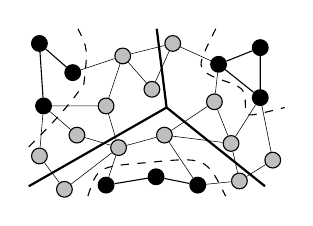
\begin{tikzpicture}
  [scale=0.5, cn/.style={circle,draw,inner sep=0,minimum size=2mm},
   p0/.style={fill},
   p1/.style={fill},
   p2/.style={fill},
   s0/.style={fill=lightgray},
   s1/.style={fill=lightgray},
   s2/.style={fill=lightgray},
   g0/.style={},
   p2p/.style={very thin},
   p2s/.style={very thin},
   s2s/.style={very thin}]
\partitiongraph
\end{tikzpicture}
}
  \subfigure[$p_i$]{
\label{sfig:part_fig:p_i}
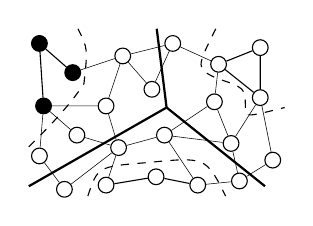
\begin{tikzpicture}
  [scale=0.5, cn/.style={circle,draw,inner sep=0,minimum size=2mm},
   p0/.style={fill},
   p1/.style={},
   p2/.style={},
   s0/.style={},
   s1/.style={},
   s2/.style={},
   g0/.style={},
   p2p/.style={very thin},
   p2s/.style={very thin},
   s2s/.style={very thin}]
\partitiongraph
\end{tikzpicture}
}
  \subfigure[$s_i$]{
\label{sfig:part_fig:s_i}
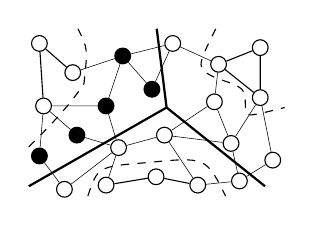
\begin{tikzpicture}
  [scale=0.5, cn/.style={circle,draw,inner sep=0,minimum size=2mm},
   p0/.style={},
   p1/.style={},
   p2/.style={},
   s0/.style={fill},
   s1/.style={},
   s2/.style={},
   g0/.style={},
   p2p/.style={very thin},
   p2s/.style={very thin},
   s2s/.style={very thin}]
\partitiongraph
\end{tikzpicture}
}
  \subfigure[$g_i$]{
\label{sfig:part_fig:g_i}
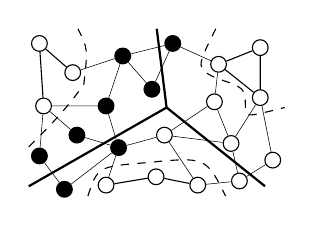
\begin{tikzpicture}
  [scale=0.5, cn/.style={circle,draw,inner sep=0,minimum size=2mm},
   p0/.style={},
   p1/.style={},
   p2/.style={},
   s0/.style={fill},
   s1/.style={},
   s2/.style={},
   g0/.style={fill},
   p2p/.style={very thin},
   p2s/.style={very thin},
   s2s/.style={very thin}]
\partitiongraph
\end{tikzpicture}
}
  \label{fig:part_fig}
  \caption{Partitions of $r{\_}all{\_}nodes$}
%  \caption[My caption
\end{figure}


%\lstset{
  captionpos=b,
  language=C++,
  basicstyle=\scriptsize,
  numbers=left,
  numberstyle=\tiny,
  columns=fullflexible,
  stepnumber=1,
  escapechar=\#,
  keepspaces=true,
  literate={<}{{$\langle$}}1 {>}{{$\rangle$}}1,
  morekeywords={region_relation,region,coloring,partition,spawn},
  deletekeywords=float,
}
\begin{lstlisting}[float={t},label={lst:code_ex},caption={Circuit Simulation Code Example}]
struct Node<rn>    { Node<rn>@rn next;    float charge, capacitance; }
struct Wire<rn,rn2,rw> { Wire<rn,rn2,rw>@rw next;
                                          Node<rn2>@rn in_node, out_node; float current, ... ; }
region_relation Circuit {
  region< Node<r_all_nodes> >                        r_all_nodes;
  region< Wire<r_all_nodes,r_all_nodes,r_all_wires> >       r_all_wires;
  Node<r_all_nodes>@r_all_nodes                   first_node;
  Wire<r_all_nodes,r_all_wires>@r_all_wires   first_wire;
}
region_relation CircuitPiece<rn, rw> {
  region< Node<rn_pvt+rn_shr> >                                 rn_pvt (#$\prec$# rn), rn_shr (#$\prec$# rn);
  region< Node<rn> >                                                   rn_ghost (#$\prec$# rn);
  region< Wire<rn_pvt+rn_shr+rn_ghost,rn,rw_pvt> >  rw_pvt (#$\prec$# rw);
  Node<rn_pvt+rn_shr>@(rn_pvt+rn_shr)                     first_node;
  Wire<rn_pvt+rn_shr+rn_ghost,rn,rw_pvt>@rw_pvt    first_wire;
};
void simulate_circuit(Circuit c) : RWE(c.r_all_nodes,c.r_all_wires)
{
  partition<c.r_all_wires> p_wires(wire_owner_map); // colored by piece they're in
  partition<c.r_all_nodes> p_nodes_pvs(node_sharing_map);
                                                                    // true = some neighbors in other pieces
  partition<p_nodes_pvs[false]> p_pvt_nodes(node_owner_map);
                                                                    // colored by piece they're in
  partition<p_nodes_pvs[true]> p_shr_nodes(node_owner_map);
                                                                    // colored by piece they're in
  partition<p_nodes_pvs[true]> p_ghost_nodes(node_nghbr_map);
                                                                    // colored by pieces they neighbor

  CircuitPiece<c.r_all_nodes,c.r_all_wires> pieces[MAX_PIECES];
  for(i = 0; i #$<$# MAX_PIECES; i++) 
    pieces[i] #$\gets$# { rn_pvt = p_pvt_nodes[i], rn_shr = p_shr_nodes[i],
                            rn_ghost = p_ghost_nodes[i], rw_pvt = p_wires[i] };

  while(!done) {
    for(i = 0; i #$<$# MAX_PIECES; i++) spawn calc_new_currents(pieces[i]);
    for(i = 0; i #$<$# MAX_PIECES; i++) spawn distribute_charge(pieces[i]);
    for(i = 0; i #$<$# MAX_PIECES; i++) spawn update_voltages(pieces[i]);
  }
}

// read info from nodes connected to each wire, update state of wire
void calc_new_currents(CircuitPiece<rn,rw> piece): RWE(piece.rw_pvt),
                                                                         ROE(piece.rn_pvt,piece.rn_ghost)

// current moving through wires redistributes charge between nodes
void distribute_charge(CircuitPiece<rn,rw> piece): ROE(piece.rw_pvt),
                                                                         RdA(piece.rn_pvt,piece.rn_ghost)

// total charge added to a node causes changes in voltage
void update_voltages(CircuitPiece<rn,rw> piece): RWE(piece.rn_pvt,piece.rn_shr)
\end{lstlisting}

%\def\partitiontree{
%\draw[step=0.5,gray,very thin] (0,0) grid (8,5);

\node(top) at (3.5,4.5) { $all{\_}nodes$ };

\node(pvsf) at (2,2.5) { $pvs[false]$ };
\node(pvst) at (5,2.5) { $pvs[true]$ };

\node(p0) at (0.7,0.5) { $p_0$ };
\node(p1) at (1.2,0.5) { $p_1$ };
\node(pd) at (1.6,0.5) { $\ldots$ };
\node(pn) at (2.3,0.5) { $p_{n-1}$ };

\node(s0) at (3.2,0.5) { $s_0$ };
\node(s1) at (3.7,0.5) { $s_1$ };
\node(sd) at (4.1,0.5) { $\ldots$ };
\node(sn) at (4.8,0.5) { $s_{n-1}$ };

\node(g0) at (5.7,0.5) { $g_0$ };
\node(g1) at (6.2,0.5) { $g_1$ };
\node(gd) at (6.6,0.5) { $\ldots$ };
\node(gn) at (7.3,0.5) { $g_{n-1}$ };

\draw[xshift=3.5cm,yshift=3.5cm] (-1,0) -- (1,0)
  node(ptf)[pos=0.25,inner sep=0] {} edge (pvsf.north)
  node[pos=0.5,anchor=south east] {$*$}
  node(ptp)[pos=0.5,inner sep=0] {} edge (top.south)
  node(ptt)[pos=0.75,inner sep=0] {} edge (pvst.north)
  ;

\draw[xshift=1.5cm,yshift=1.5cm] (-1,0) -- (1,0)
  node(pp0)[pos=0.2,inner sep=0] {} edge (p0.north)
  node(pp1)[pos=0.4,inner sep=0] {} edge (p1.north)
  node[pos=0.5,anchor=south east] {$*$}
  node(ppp)[pos=0.5,inner sep=0] {} edge (pvsf.250)
  node(ppn)[pos=0.8,inner sep=0] {} edge (pn.north)
  ;

\draw[xshift=4cm,yshift=1.5cm] (-1,0) -- (1,0)
  node(ps0)[pos=0.2,inner sep=0] {} edge (s0.north)
  node(ps1)[pos=0.4,inner sep=0] {} edge (s1.north)
  node[pos=0.5,anchor=south east] {$*$}
  node(psp)[pos=0.5,inner sep=0] {} edge (pvst.230)
  node(psn)[pos=0.8,inner sep=0] {} edge (sn.north)
  ;

\draw[xshift=6.5cm,yshift=1.5cm] (-1,0) -- (1,0)
  node(pg0)[pos=0.2,inner sep=0] {} edge (g0.north)
  node(pg1)[pos=0.4,inner sep=0] {} edge (g1.north)
  node[pos=0.5,anchor=south east] {}
  node(pgp)[pos=0.5,inner sep=0] {} edge (pvst.310)
  node(pgn)[pos=0.8,inner sep=0] {} edge (gn.north)
  ;
}

\def\partitiongraph{
%\draw[step=0.5,gray,very thin] (0,0) grid (8,5);

\node[cn,s0] (n1) at (0.77,1.27) {};
\node[cn,p0] (n2) at (1.6165,3.3865) {};
\node[cn,s0] (n3) at (2.463,2.54) {};
\node[cn,p0] (n4) at (0.8755,2.54) {};
\node[cn,p2] (n5) at (2.463,0.529) {};
\node[cn,s2] (n6) at (3.945,1.799) {};
\node[cn,s0] (n7) at (3.6275,2.963) {};
\node[cn,p2] (n8) at (4.7915,0.529) {};
\node[cn,s1] (n9) at (5.638,1.5875) {};
\node[cn,s1] (n10) at (6.6965,1.164) {};
\node[cn,s1] (n11) at (5.215,2.6455) {};
\node[cn,p1] (n12) at (6.379,2.7515) {};
\node[cn,p1] (n13) at (5.3205,3.598) {};
\node[cn,s1,g0] (n14) at (4.1565,4.1275) {};
\node[cn,s0] (n15) at (2.8865,3.81) {};
\node[cn,p0] (n16) at (0.77,4.1275) {};
\node[cn,s2,g0] (n17) at (1.405,0.423) {};
\node[cn,p1] (n18) at (6.379,4.0215) {};
\node[cn,s2,g0] (n19) at (2.7805,1.4815) {};
\node[cn,s0] (n20) at (1.7225,1.799) {};
\node[cn,p2] (n21) at (3.733,0.7405) {};
\node[cn,s2] (n22) at (5.85,0.635) {};

\draw (n16) to (n2);
\draw (n16) to (n4);
\draw (n5) to (n21);
\draw (n21) to (n8);
\draw (n12) to (n13) to (n18) to (n12);


\draw[p2s] (n1) to (n4) to (n20);
\draw[p2s] (n4) to (n3) to (n15) to (n2);
\draw[p2s] (n15) to (n7);

\draw[p2s] (n14) to (n13) to (n11) to (n9) to (n12) to (n10);

\draw[p2s] (n17) to (n19) to (n5);
\draw[p2s] (n19) to (n6) to (n8) to (n22);

\draw[s2s] (n1) to (n17);
\draw[s2s] (n20) to (n19) to (n3);
\draw[s2s] (n15) to (n14) to (n7);
\draw[s2s] (n11) to (n6) to (n9) to (n22) to (n10);

\draw[thick] (0.5,0.5) to (4,2.5);
\draw[thick] (3.75,4.5) to (4,2.5);
\draw[thick] (6.5,0.5) to (4,2.5);

\draw[dashed] (0.5,1.5) .. controls (1,2) and (1.5,2.5) .. (1.9,3.1) .. controls (2,4) .. (1.75,4.5);
\draw[dashed] (5.25,4.5) .. controls (4.75,3.5) .. (5.25,3.25) .. controls (6,3) .. (6,2.5) .. controls (6,2.25) .. (7,2.5);
\draw[dashed] (2,0.25) .. controls (2.25,1) .. (3.5,1.1) .. controls (5,1.25) .. (5.5,0.25);
}

\begin{figure}[t]
  \centering
\subfigure[partitioning tree]{
\label{sfig:part_fig:tree}
\begin{tikzpicture}[scale=0.8]
\partitiontree
\end{tikzpicture}
}

  \subfigure[$pvs$]{
\label{sfig:part_fig:pvs}
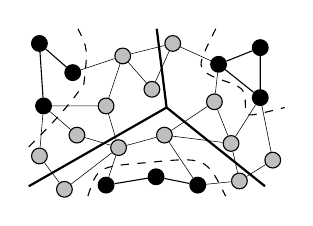
\begin{tikzpicture}
  [scale=0.5, cn/.style={circle,draw,inner sep=0,minimum size=2mm},
   p0/.style={fill},
   p1/.style={fill},
   p2/.style={fill},
   s0/.style={fill=lightgray},
   s1/.style={fill=lightgray},
   s2/.style={fill=lightgray},
   g0/.style={},
   p2p/.style={very thin},
   p2s/.style={very thin},
   s2s/.style={very thin}]
\partitiongraph
\end{tikzpicture}
}
  \subfigure[$p_i$]{
\label{sfig:part_fig:p_i}
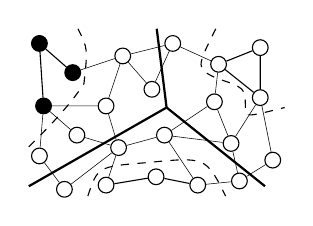
\begin{tikzpicture}
  [scale=0.5, cn/.style={circle,draw,inner sep=0,minimum size=2mm},
   p0/.style={fill},
   p1/.style={},
   p2/.style={},
   s0/.style={},
   s1/.style={},
   s2/.style={},
   g0/.style={},
   p2p/.style={very thin},
   p2s/.style={very thin},
   s2s/.style={very thin}]
\partitiongraph
\end{tikzpicture}
}
  \subfigure[$s_i$]{
\label{sfig:part_fig:s_i}
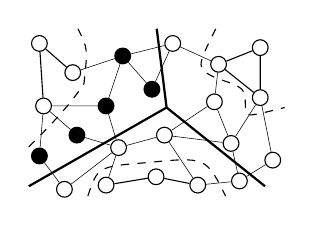
\begin{tikzpicture}
  [scale=0.5, cn/.style={circle,draw,inner sep=0,minimum size=2mm},
   p0/.style={},
   p1/.style={},
   p2/.style={},
   s0/.style={fill},
   s1/.style={},
   s2/.style={},
   g0/.style={},
   p2p/.style={very thin},
   p2s/.style={very thin},
   s2s/.style={very thin}]
\partitiongraph
\end{tikzpicture}
}
  \subfigure[$g_i$]{
\label{sfig:part_fig:g_i}
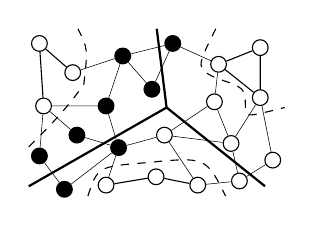
\begin{tikzpicture}
  [scale=0.5, cn/.style={circle,draw,inner sep=0,minimum size=2mm},
   p0/.style={},
   p1/.style={},
   p2/.style={},
   s0/.style={fill},
   s1/.style={},
   s2/.style={},
   g0/.style={fill},
   p2p/.style={very thin},
   p2s/.style={very thin},
   s2s/.style={very thin}]
\partitiongraph
\end{tikzpicture}
}
  \label{fig:part_fig}
  \caption{Partitions of $r{\_}all{\_}nodes$}
%  \caption[My caption
\end{figure}

